\documentclass[12pt,fleqn]{article}\usepackage{../common}
\begin{document}
Gaussian Olcumlerin Fuzyonu (Gaussian Sensor Fusion)

Tek boyutlu ortamda bir buyuklugu mesela bir lokasyon bilgisi $x$'i, iki
kere olcuyoruz, ve bu olcumu iki degisik algilayiciya yaptiriyoruz, ve yine
diyelim ki iki degisik alet bir cismin oldugu uzakligini / yerini bize geri
donduruyor. Devam edelim, bu bilgilerde belli olcude gurultu var; bu
aletlerin hatali olcumu yuzunden olabilir, cevre sartlari sebebiyle
olabilir, ornek olarak iki $z_1,z_2$ olcumu icin iki degisik belirsizlik
(uncertainty) oldugunu farzedelim, bunlar $\sigma_1,\sigma_2$. Soru su: bu
iki olcumu kullanarak daha iyi bir $x$ tahmini yapabilir miyiz?

Bunun icin iki olcumu bir sekilde birlestirmemiz gerekiyor. Her olcumu
Gaussian / Normal dagilim olarak modelleyebiliriz, o zaman iki Gaussian
dagilimi bir sekilde birlestirmemiz (fusion) lazim. 

Olcumleri temsil etmek icin Gaussian bicilmis kaftan. Olcumdeki
belirsizligi standart sapma (standart deviation) uzerinden rahatlikla
temsil edebiliriz. Peki birlestirimi nasil yapalim?

Bu tur problemlerde maksimum olurluk (maximum likelihood) kullanilmasi
gerektigini asagi yukari tahmin edebiliriz, cunku maksimum olurluk verinin
olurlugunu (olasiligini yani) maksimize ederek bilinmeyen parametreleri
tahmin etmeye ugrasir. Cogunlukla bu teknigi hep {\em tek} bir dagilim
baglaminda goruruz, bazi bilinmeyen parametreleri olan tek bir dagilima
degisik veri noktalari verilerek olasilik sonuclari carpilir, ve elde
edilen formul maksimize edilmeye ugrasilirken ayni anda bilinmeyen
parametrelerin optimal degerleri saptanmaya ugrasilir. Bizim bu
problemimizde iki degisik dagilim olacak, maksimum olurluk illa tek bir
dagilimla kullanilabilir diye bir kural yok.

Problemimizde iki olcumu, iki Gaussian ile temsil edebiliriz, ve bu iki
Gaussian'a verilen iki olcum noktasini olurlugunu bu Gaussian'larin
sonuclarini carparak hesaplayabiliriz. Peki bilinmeyen parametre nedir? Onu
da {\em her iki Gaussian icin de ayni oldugunu farzettigimiz orta nokta}
(mean) olarak alabiliriz, ve $x$ olarak belirtiriz. Yani

$$ L(x) = p(z_1|x,\sigma_1) p(z_2|x,\sigma_2) $$

$$ L(x) \sim \exp{\frac{-(z_1-x)^2}{2\sigma_1^2} } 
\times \exp \frac{-(z_2-x)^2}{2\sigma_2^2} $$

1D Gaussian formulunu hatirlarsak, 

$$ p(z;x,\sigma) = \frac{1}{\sigma\sqrt{2\pi}} 
\exp \bigg\{ - \frac{(z-x)^2}{2\sigma^2}  \bigg\}
 $$

Ders notlari [1]'de iki ustteki formulun nasil maksimize edilerek bir
$x_{MLE}$ formulune erisildigini gorebiliriz. 

Formul basindaki sabit kisminin $L(x)$'de kullanilmadigini goruyoruz, cunku
maksimizasyon acisindan dusunursek o kisim tekrar tekrar carpilacak ve
hesaplamaya calistigimiz degiskenler acisindan bu surekli tekrar bir
fark yaratmaz.

Bu metot isler. Fakat biz alternatif olarak daha temiz olacak degisik bir
yoldan gidecegiz. Elimizdeki her iki olcumu iki farkli tek boyutlu Gaussian
yerine {\em 2 boyutlu} tek bir Gaussian icine koyacagiz, iki olcumu tek
bir 2 boyutlu vektor icinde belirtecegiz yani, ve tek bir olasilik hesabini
$p(z;x,\Sigma)$'i baz alacagiz.  Belirsizlikler ne olacak? Olcum
belirsizliklerini bu 2D Gaussian'in kovaryansinda capraza (diagonal)
koyabiliriz, capraz disindaki matris ogeleri sifir yapilirsa iki olcumun
birbirinden bagimsizligini temsil etmis oluruz. Maksimizasyon? Tek bir
olcumun olurlugunu maksimize edecegiz, bu tek bir olcumun olasiligini
hesaplamaktan ibarettir, ve bu hesap sirasinda bilinmeyen degiskenleri
iceren yeni bir formul ortaya cikacaktir. Maksimize etmeye ugrasacagimiz bu
formul olur.

Cok boyutlu Gaussian'i hatirlayalim (artik $z,x$ birer vektor),

$$ p(z;x,\Sigma) = 
\frac{ 1}{(2\pi)^{k/2} \det(\Sigma)^{1/2}} \exp 
\bigg\{ 
-\frac{ 1}{2}(z-x)^T\Sigma^{-1}(z-x)
\bigg\} $$

Kisaca,

$$ =  \frac{ 1}{C} \exp 
\bigg\{ 
-\frac{ 1}{2}(z-x)^T\Sigma^{-1}(z-x)
\bigg\} $$

Bir numara, $\exp$ ve parantez ici negatif ibareden kurtulmak icin
$-\ln p$ alalim,

$$ L = -\ln p(z) = 
\frac{ 1}{2}(z-x)^T\Sigma^{-1}(z-x)
$$

Simdi iki olcumu, belirsizligi vektor / matris ogeleri olarak gosterelim, 

$$ = \frac{1}{2}  
\left[\begin{array}{c}
z_1-x \\ z_2-x
\end{array}\right]^T
\left[\begin{array}{cc}
\sigma_1^2 & 0 \\
0 & \sigma_2^2 
\end{array}\right]^{-1}
\left[\begin{array}{c}
z_1-x \\ z_2-x
\end{array}\right]
$$

Capraz matrisin tersini almak icin caprazdaki ogelerin tersini almak
yeterlidir,

$$ = \frac{1}{2}  
\left[\begin{array}{c}
z_1-x \\ z_2-x
\end{array}\right]^T
\left[\begin{array}{cc}
\sigma_1^{-2} & 0 \\
0 & \sigma_2^{-2} 
\end{array}\right]
\left[\begin{array}{c}
z_1-x \\ z_2-x
\end{array}\right]
$$

$$ = \frac{1}{2}  
\left[\begin{array}{cc}
\sigma_1^{-2}(z_1-x) & \sigma_2^{-2} (z_2-x)
\end{array}\right]
\left[\begin{array}{c}
z_1-x \\ z_2-x
\end{array}\right]
$$

$$ = 
\frac{1}{2}\sigma_1^{-2}(z_1-x)^2 + \frac{1}{2}\sigma_2^{-2} (z_2-x)^2
$$

Maksimize etmek icin, formul karesel olduguna gore, bilinmeyen $x$
degiskenine gore turev alip sifira esitleyebiliriz,

$$ 
\frac{dL}{dx} = \sigma_1^{-2}z_1-\sigma_1^{-2}x + \sigma_2^{-2}z_2-\sigma_2^{-2}x = 0
$$

$x$ uzerinden gruplarsak,

$$ 
-x(\sigma_1^{-2}+\sigma_2^{-2}) + \sigma_1^{-2}z_1+ \sigma_2^{-2}z_2 = 0
$$

Gruplanan kismi esitligin sagina alalim,

$$ 
\sigma_1^{-2}z_1+ \sigma_2^{-2}z_2 = x(\sigma_1^{-2}+\sigma_2^{-2}) 
$$

$$ 
\frac{\sigma_1^{-2}z_1+ \sigma_2^{-2}z_2 }{\sigma_1^{-2}+\sigma_2^{-2}}= x_{MLE}
$$

Gayet temiz bir sekilde sonuca eristik. 

Ornek

Elimizde belirsizlikleri $\sigma_1=10,\sigma_2=20$ olan iki algilayici
var. Bu algilayicilar ayni obje hakkinda $z_1=130,z_2=170$ olarak iki olcum
gonderiyorlar. Bu olcumleri birlestirelim. Hatirlarsak $10^{-2}$ ile
carpmak $10^{2}$ ile bolmek ayni sey.

$$ x_{MLE} =
\frac{130/10^2 + 170/20^2}{1/10^2 + 1/20^2} = 138.0
$$

Sonuc belirsizligi daha az olan olcume daha yakin cikti, bu akla yatkin
bir sonuc.

Cok Boyutlu Gaussian Fuzyon

Peki ya elimizdeki olcumlerin kendisi cok boyutlu ise? Yani $z_1,z_2$ birer
vektor ise?

Yine maksimum olurluk uzerinden bir formul turetebiliriz. Bu durumda tek
olasilik hesabi yetmez, iki ayri dagilim olmali,

$$ p(z_1;x,\Sigma_1) =  \frac{ 1}{C_1} \exp 
\bigg\{ 
-\frac{ 1}{2}(z_1-x)^T\Sigma_1^{-1}(z_1-x)
\bigg\} $$

$$ p(z_2;x,\Sigma_2) =  \frac{ 1}{C_2} \exp 
\bigg\{ 
-\frac{ 1}{2}(z_2-x)^T\Sigma_2^{-1}(z_2-x)
\bigg\} $$

Orta nokta $x$ her iki formulde ayni cunku degismeyen olan o; ayni orta
nokta icin tahmin uretmeye ugrasiyoruz. Bu durum bildik maksimum olurluk
hesaplarina benziyor, fakat ilk basta belirttigimiz gibi farkli turden
olasilik fonksiyonlarinin (bu sefer cok boyutlu) farkli veri noktalari
uzerinden carpilmasi.

Devam edelim. Daha once $\ln$ alarak $\exp$'yi yoketmistik. Bunun bir diger
faydasi $\ln$ alininca carpimlarin toplama donusmesidir, 

$$ L = p(z_1;x,\Sigma_1) p(z_2;x,\Sigma_2) 
$$

$$ -\ln L = -\ln p(z_1;x,\Sigma_1) -\ln p(z_2;x,\Sigma_2) 
$$

$$ 
\mathcal{L} = 
-\ln L = 
\frac{ 1}{2}(z_1-x)^T\Sigma_1^{-1}(z_1-x) + 
\frac{ 1}{2}(z_2-x)^T\Sigma_2^{-1}(z_2-x)
$$

Simdi esitligin sag tarafinin $x$'e gore turevini alalim, vektor ve matris
baglaminda turev nasil alinir? Herhangi bir $M$'in simetrik oldugu
durumlarda (ki kovaryans matrisleri her zaman simetriktir, cunku mesela iki
degiskenli durumda $x_1,x_2$ kovaryansi -iliskisi- $x_2,x_1$ kovaryansindan
farkli olamaz),

$$ \frac{\partial}{\partial x}[x^TMx] = 2Mx $$

oldugunu biliyoruz [2]. O zaman turev sonucu soyle olur, 

$$ 
\frac{d\mathcal{L}}{dx} = 
(z_1-x)^T\Sigma_1^{-1} +  (z_2-x)^T\Sigma_2^{-1}
$$

Sifira esitleyip cozelim, 

$$ 
(z_1-x)\Sigma_1^{-1} +  (z_2-x)\Sigma_2^{-1} = 0
$$

$$ 
z_1\Sigma_1^{-1} - x\Sigma_1^{-1} + z_2\Sigma_2^{-1} - x\Sigma_2^{-1} = 0
$$

Yine $x$ altinda gruplayalim,

$$ 
-x(\Sigma_1^{-1} + \Sigma_2^{-1}) + z_1\Sigma_1^{-1}  + z_2\Sigma_2^{-1}  = 0
$$

$$ 
z_1\Sigma_1^{-1}  + z_2\Sigma_2^{-1}  = x(\Sigma_1^{-1} + \Sigma_2^{-1}) 
$$

Eger iki belirsizligin toplamini $\Sigma_x^{-1}$ olarak ozetlersek, yani 

$$ 
\Sigma_x^{-1} = \Sigma_1^{-1} + \Sigma_2^{-1}
$$

Not: Aslinda $\Sigma_x$ te diyebilirdik, fakat tersi alinmis matrislerin
toplami oldugunu temsil etmesi icin ``tersi alinmis bir sembol''
kullandik. Tabii diger yandan tersin tersini alinca ele gececek
$\Sigma_x$'in de bir anlami oldugu iddia edilebilir, bu $\Sigma_x$ en olasi
$x$ tahmininin yeni belirsizligidir de bir bakima. 

Simdi ana formule donelim,

$$ 
z_1\Sigma_1^{-1}  + z_2\Sigma_2^{-1}  = x\Sigma_x^{-1}
$$


$$ 
\Sigma_x (z_1\Sigma_1^{-1}  + z_2\Sigma_2^{-1}) = x_{MLE}
$$

Ornek

Elimizde iki tane iki boyutlu olcum var, 

$$ z_1 = \left[\begin{array}{c}
1 \\ 1
\end{array}\right], 
z_2 = \left[\begin{array}{r}
2 \\ -1
\end{array}\right] 
$$

Olcumler iki degisik algilayicidan geliyor, belirsizlikleri

$$ 
\Sigma_1 = 
\left[\begin{array}{cc}
1 & 0 \\ 0 & 4
\end{array}\right], 
\Sigma_2 = 
\left[\begin{array}{cc}
4 & 0 \\ 0 & 1
\end{array}\right]
 $$

Nihai olcum nedir? 

\begin{minted}[fontsize=\footnotesize]{python}
from mpl_toolkits.mplot3d import Axes3D
from matplotlib import cm
import matplotlib.mlab as mlab

x = np.arange(-10.0, 10.0, 0.1)
y = np.arange(-10.0, 10.0, 0.1)

X, Y = np.meshgrid(x, y)
Z1 = mlab.bivariate_normal(X, Y, sigmax=1.0, sigmay=4.0,mux=1., \
     muy=1.,sigmaxy=0.0)
Z2 = mlab.bivariate_normal(X, Y, sigmax=4.0, sigmay=1.0,mux=2., \
     muy=-1.,sigmaxy=0.0)

# iki yuzeyi ayni grafikte birlestirmek icin herhangi iki nokta arasinda
# daha fazla (maksimum) olani al, cunku nihai yuzey olarak onu gormek 
# istiyoruz zaten
Z = np.maximum(Z1,Z2)

fig = plt.figure()

ax = Axes3D(fig)
ax.view_init(elev=50., azim=80)

ax.plot_surface(X,Y,Z,cmap=cm.jet)
plt.savefig('fusion_1.png')
\end{minted}


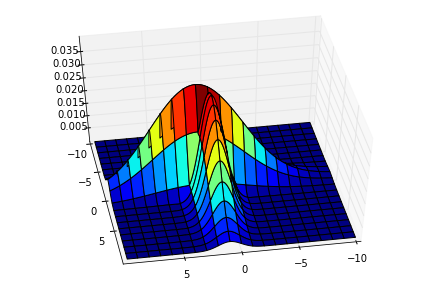
\includegraphics[height=6cm]{fusion_1.png}

Iki olcumu Gaussian olarak ekrana bastik, bu Gaussian'larin orta noktasi
$z_1,z_2$, bu durumu maksimum olurluk icin ayni oldugunu farz ettigimiz $x$
ile karistirmayalim; o $x$ modelleme sirasinda oldugunu farzettigimiz ideal
bir Gaussian idi. Ustte sadece veri noktalarini ekrana basiyoruz. 


Ustten bakisla kontur (contour) olarak gosterirsek 

\begin{minted}[fontsize=\footnotesize]{python}
CS = plt.contour(X, Y, Z1,rotation=70)
CS = plt.contour(X, Y, Z2,rotation=70)
plt.savefig('fusion_3.png')
\end{minted}

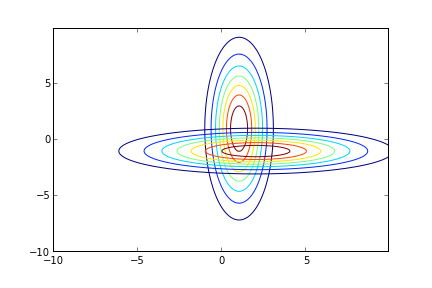
\includegraphics[height=6cm]{fusion_3.png}


Resimde once ilk olcum, sonra onunla yanyana olacak ikinci olcum koyulmus. 

$$ \Sigma_x^{-1} = \Sigma_1^{-1} + \Sigma_2^{-1}  =
\left[\begin{array}{cc}
1 & 0 \\ 0 & 0.25
\end{array}\right] + 
\left[\begin{array}{cc}
0.25 & 0 \\ 0 & 1
\end{array}\right] =
\left[\begin{array}{cc}
1.25 & 0 \\ 0 & 1.25
\end{array}\right] 
$$

Tersini alalim 

$$ \Sigma_x =
\left[\begin{array}{cc}
0.8 & 0 \\ 0 & 0.8
\end{array}\right] 
$$

$$ x_{MLE} =  \Sigma_x (z_1\Sigma_1^{-1}  + z_2\Sigma_2^{-1}) $$

$$ 
x_{MLE} =
\left[\begin{array}{cc}
0.8 & 0 \\ 0 & 0.8
\end{array}\right] 
\bigg(
\left[\begin{array}{cc}
1 & 0 \\ 0 & 0.25
\end{array}\right] 
\left[\begin{array}{c}
1 \\ 1
\end{array}\right]  + 
\left[\begin{array}{cc}
0.25 & 0 \\ 0 & 1
\end{array}\right] 
\left[\begin{array}{r}
2 \\ -1
\end{array}\right]  
\bigg) = 
\left[\begin{array}{r}
1.2 \\ -0.6
\end{array}\right]  
$$

Sonuc grafiklenirse suna benzer (ki yeni belirsizlik $\Sigma_x$'i de
grafikte kullanalim),

\begin{minted}[fontsize=\footnotesize]{python}
Z3 = mlab.bivariate_normal(X, Y, sigmax=0.8, sigmay=0.8,mux=1.2, \
     muy=-0.6,sigmaxy=0.0)

fig = plt.figure()

ax = Axes3D(fig)
ax.view_init(elev=40.,azim=80)

ax.plot_surface(X,Y,Z3,cmap=cm.jet)
plt.savefig('fusion_2.png')
\end{minted}



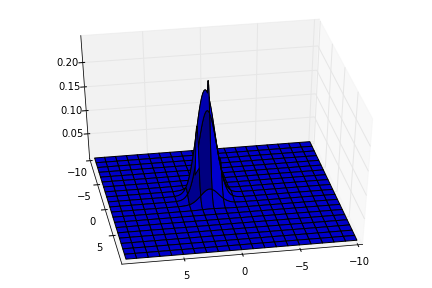
\includegraphics[height=6cm]{fusion_2.png}

Yeni tahminimiz boyle cikti. Cok daha emin oldugumuz bir noktada en olasi
olcumu ortaya cikardik. Kontur olarak grafiklersek,

\begin{minted}[fontsize=\footnotesize]{python}
CS = plt.contour(X, Y, Z3)
plt.savefig('fusion_4.png')
\end{minted}

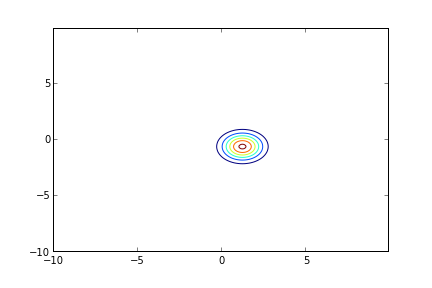
\includegraphics[height=6cm]{fusion_4.png}


[1] \url{www.robots.ox.ac.uk/~az/lectures/est/lect34.pdf}

[2] Hart, Duda, {\em Pattern Classification}

\end{document}
